\documentclass[12pt,a4paper]{article}

% ── Packages ──────────────────────────────────────────────
\usepackage[margin=1in]{geometry}
\usepackage{times}
\usepackage{graphicx}
\usepackage{booktabs}
\usepackage{enumitem}
\usepackage{hyperref}
\usepackage{xcolor}
\usepackage{titlesec}
\usepackage{fancyhdr}
\usepackage{setspace}
\usepackage{caption}
\usepackage{array}
\usepackage{tabularx}
\usepackage{listings}
\usepackage{float}

% ── Colors ────────────────────────────────────────────────
\definecolor{snapblue}{HTML}{0D1525}
\definecolor{snapcyan}{HTML}{00C2FF}
\definecolor{codebg}{HTML}{F1F5F9}
\definecolor{codetext}{HTML}{1E293B}

% ── Code Listing Style ───────────────────────────────────
\lstset{
    backgroundcolor=\color{codebg},
    basicstyle=\ttfamily\small\color{codetext},
    keywordstyle=\color{blue}\bfseries,
    commentstyle=\color{gray}\itshape,
    stringstyle=\color{red!70!black},
    breaklines=true,
    frame=single,
    rulecolor=\color{gray!30},
    numbers=left,
    numberstyle=\tiny\color{gray},
    tabsize=4,
    showstringspaces=false
}

% ── Header/Footer ────────────────────────────────────────
\pagestyle{fancy}
\fancyhf{}
\fancyhead[L]{\small\textcolor{gray}{SnapPark Enhancement Report}}
\fancyhead[R]{\small\textcolor{gray}{Levinesh G R}}
\fancyfoot[C]{\thepage}
\renewcommand{\headrulewidth}{0.4pt}

% ── Section Formatting ───────────────────────────────────
\titleformat{\section}{\Large\bfseries\color{snapblue}}{}{0em}{}[\titlerule]
\titleformat{\subsection}{\large\bfseries\color{snapblue!80}}{}{0em}{}

% ── Line Spacing ─────────────────────────────────────────
\setstretch{1.3}

\begin{document}

% ══════════════════════════════════════════════════════════
%  COVER PAGE
% ══════════════════════════════════════════════════════════
\begin{titlepage}
    \centering
    \vspace*{2cm}
    
    {\Huge\bfseries\textcolor{snapblue}{SnapPark}\par}
    \vspace{0.3cm}
    {\Large\textcolor{snapcyan}{Smart Parking Management System}\par}
    
    \vspace{1.5cm}
    \rule{\textwidth}{1.5pt}
    \vspace{0.5cm}
    
    {\LARGE\bfseries Enhancement Report\par}
    \vspace{0.3cm}
    {\Large\textcolor{snapblue}{Monthly Vehicle Visit Frequency PDF Report}\par}
    
    \vspace{0.5cm}
    \rule{\textwidth}{1.5pt}
    
    \vspace{2cm}
    
    \begin{tabular}{ll}
        \textbf{Student Name}    & Levinesh G R \\
        \textbf{Role}            & Backend Developer \& Report Module \\
        \textbf{Course}          & B.Tech Computer Science \\
        \textbf{Department}      & School of Computer Engineering \& Technology \\
        \textbf{College}         & MIT World Peace University, Pune \\
        \textbf{Guide}           & Professor Suhas Joshi \\
    \end{tabular}
    
    \vspace{2cm}
    
    {\large\textbf{Submission Date:} 27th April 2026\par}
    
    \vfill
    {\small\textcolor{gray}{Java 21 $\cdot$ JavaFX $\cdot$ PostgreSQL $\cdot$ OpenPDF $\cdot$ Embedded HTTP Server}\par}
\end{titlepage}

% ══════════════════════════════════════════════════════════
%  ABSTRACT
% ══════════════════════════════════════════════════════════
\newpage
\section*{Abstract}
\addcontentsline{toc}{section}{Abstract}

The SnapPark system collects rich data about vehicle visits through its \texttt{parking\_sessions} table, but the original system lacked any reporting or analytics export capability. Administrators had no way to analyze visit patterns, identify frequent customers, or generate reports for management review.

This enhancement introduces a \textbf{Monthly Vehicle Visit Frequency PDF Report} system that aggregates parking session data by vehicle and month, generating professionally branded PDF documents. The system spans the full MVC stack: a \texttt{ReportDAO} for SQL aggregation queries, a \texttt{PdfReportService} using the OpenPDF library for document generation, a REST API endpoint for programmatic access, and JavaFX UI controls for one-click downloads from the Analytics dashboard. The report includes vehicle numbers, phone numbers, vehicle types, visit counts sorted by frequency, and a total visits summary.

% ══════════════════════════════════════════════════════════
%  TABLE OF CONTENTS
% ══════════════════════════════════════════════════════════
\newpage
\tableofcontents
\newpage

% ══════════════════════════════════════════════════════════
%  SECTION 1: INTRODUCTION
% ══════════════════════════════════════════════════════════
\section{Introduction}

\subsection{Background}
SnapPark stores all parking sessions in a PostgreSQL database with timestamps, vehicle references, and billing information. However, the original system provided no way to extract, analyze, or export this data. Administrators could view real-time slot status but had no historical reporting capability.

Key limitations:
\begin{itemize}[noitemsep]
    \item No way to identify frequently returning vehicles
    \item No exportable reports for management or auditing
    \item No monthly aggregation or trend analysis
    \item No API for external systems to fetch report data
\end{itemize}

\subsection{Objectives}
\begin{enumerate}[noitemsep]
    \item Create a DTO (Data Transfer Object) for report data rows.
    \item Build a DAO with SQL JOIN + GROUP BY + COUNT aggregation.
    \item Generate branded PDF reports using the OpenPDF library.
    \item Expose a REST API endpoint for programmatic PDF download.
    \item Add JavaFX UI controls (ComboBoxes + Button) for admin access.
    \item Handle edge cases: empty data, invalid dates, generation failures.
\end{enumerate}

\subsection{Enhancement Summary}

\begin{table}[H]
\centering
\caption{PDF Report — Feature Summary}
\begin{tabularx}{\textwidth}{|l|X|}
\hline
\textbf{Area} & \textbf{Features} \\
\hline
Model Layer & \texttt{VehicleFrequencyRow} DTO (immutable, 4 fields) \\
\hline
DAO Layer & \texttt{ReportDAO.getMonthlyFrequency()} with JOIN + GROUP BY \\
\hline
Service Layer & \texttt{PdfReportService} — branded PDF generation with OpenPDF \\
\hline
API Layer & \texttt{GET /api/report/frequency?year=\&month=} \\
\hline
UI Layer & Analytics tab with month/year pickers and download button \\
\hline
Dependency & OpenPDF 1.3.30 added to \texttt{pom.xml} \\
\hline
\end{tabularx}
\end{table}

% ══════════════════════════════════════════════════════════
%  SECTION 2: IMPLEMENTATION
% ══════════════════════════════════════════════════════════
\section{Implementation Details}

\subsection{Architecture — Clean Layer Separation}
The report feature follows a strict layered architecture:

\begin{center}
\begin{tabular}{rcl}
\textbf{FXML UI} & $\rightarrow$ & \textbf{AnalyticsController} \\
& $\rightarrow$ & \textbf{PdfReportService} \\
& $\rightarrow$ & \textbf{ReportDAO} \\
& $\rightarrow$ & \textbf{PostgreSQL Database} \\
\end{tabular}
\end{center}

Each layer has a single responsibility: UI handles user input, Controller coordinates, Service generates PDFs, DAO executes SQL.

\subsection{Data Transfer Object — VehicleFrequencyRow.java}

\begin{lstlisting}[language=Java, caption={VehicleFrequencyRow DTO}]
public class VehicleFrequencyRow {
    private final String licensePlate;
    private final String phoneNumber;
    private final String vehicleType;
    private final int    frequency;

    public VehicleFrequencyRow(String licensePlate, 
        String phoneNumber, String vehicleType, int frequency) {
        this.licensePlate = licensePlate;
        this.phoneNumber  = phoneNumber;
        this.vehicleType  = vehicleType;
        this.frequency    = frequency;
    }
    // Getters only (immutable)
}
\end{lstlisting}

All fields are \texttt{final}---this follows the \textbf{Immutable Object Pattern}, ensuring thread safety when passed between layers.

\subsection{DAO Layer — ReportDAO.java}

\begin{lstlisting}[language=Java, caption={Monthly Frequency SQL Query}]
public List<VehicleFrequencyRow> getMonthlyFrequency(
        int year, int month) {
    String monthPrefix = String.format("%04d-%02d", year, month);
    
    String sql = "SELECT v.license_plate, v.phone_number, "
        + "v.vehicle_type, COUNT(ps.id) AS freq "
        + "FROM parking_sessions ps "
        + "JOIN vehicles v ON v.id = ps.vehicle_id "
        + "WHERE ps.entry_time LIKE ? "
        + "GROUP BY v.id, v.license_plate, "
        + "v.phone_number, v.vehicle_type "
        + "ORDER BY freq DESC, v.license_plate ASC";
    
    ps.setString(1, monthPrefix + "%");
    // Execute and map to VehicleFrequencyRow list
}
\end{lstlisting}

\textbf{SQL Concepts Used:}
\begin{itemize}[noitemsep]
    \item \texttt{JOIN} — Combines sessions with vehicle details
    \item \texttt{GROUP BY} — Aggregates sessions per vehicle
    \item \texttt{COUNT()} — Counts visit frequency
    \item \texttt{ORDER BY} — Sorts by frequency descending
    \item \texttt{LIKE} — Filters by month prefix pattern matching
    \item \texttt{PreparedStatement} — Prevents SQL injection
\end{itemize}

\subsection{Service Layer — PdfReportService.java}
The PDF is generated using the \textbf{OpenPDF} library (LGPL-licensed iText fork):

\begin{lstlisting}[language=Java, caption={PDF Generation Core Logic}]
public byte[] generateMonthlyFrequencyReport(int year, int month) {
    List<VehicleFrequencyRow> rows = 
        reportDAO.getMonthlyFrequency(year, month);
    
    Document doc = new Document(PageSize.A4, 40, 40, 40, 40);
    ByteArrayOutputStream baos = new ByteArrayOutputStream();
    PdfWriter.getInstance(doc, baos);
    doc.open();
    
    // 1. Branded header (dark bg, cyan title)
    // 2. Data table (5 columns, alternating rows)
    // 3. Total row (green background)
    // 4. Footer (generation notice)
    
    doc.close();
    return baos.toByteArray(); // PDF as byte array
}
\end{lstlisting}

\textbf{PDF Structure:}
\begin{enumerate}[noitemsep]
    \item \textbf{Header:} Dark navy background (\texttt{\#0D1525}), SnapPark branding, cyan accent title, metadata (period, timestamp, vehicle count)
    \item \textbf{Table:} 5 columns (\#, Vehicle Number, Phone, Type, Visits) with alternating row colors
    \item \textbf{Total Row:} Green background with sum of all visits
    \item \textbf{Footer:} Italic text explaining data source
\end{enumerate}

\subsection{API Endpoint — WebServer.java}

\begin{lstlisting}[language=Java, caption={REST API for PDF Download}]
// GET /api/report/frequency?year=2026&month=4
private void handleFrequencyReport(HttpExchange ex) {
    int year  = Integer.parseInt(params.get("year"));
    int month = Integer.parseInt(params.get("month"));
    
    byte[] pdf = pdfReportService
        .generateMonthlyFrequencyReport(year, month);
    
    ex.getResponseHeaders().set("Content-Type", 
        "application/pdf");
    ex.getResponseHeaders().set("Content-Disposition",
        "attachment; filename=\"...-report.pdf\"");
    ex.sendResponseHeaders(200, pdf.length);
    ex.getResponseBody().write(pdf);
}
\end{lstlisting}

\subsection{JavaFX UI — AnalyticsController + analytics.fxml}
The Analytics tab includes month/year ComboBoxes and a download button. PDF generation runs on a \textbf{background thread} to avoid freezing the UI, with \texttt{Platform.runLater()} for thread-safe UI updates.

% ══════════════════════════════════════════════════════════
%  SECTION 3: OUTPUT / SCREENSHOTS
% ══════════════════════════════════════════════════════════
\section{Output and Screenshots}

\begin{figure}[H]
    \centering
    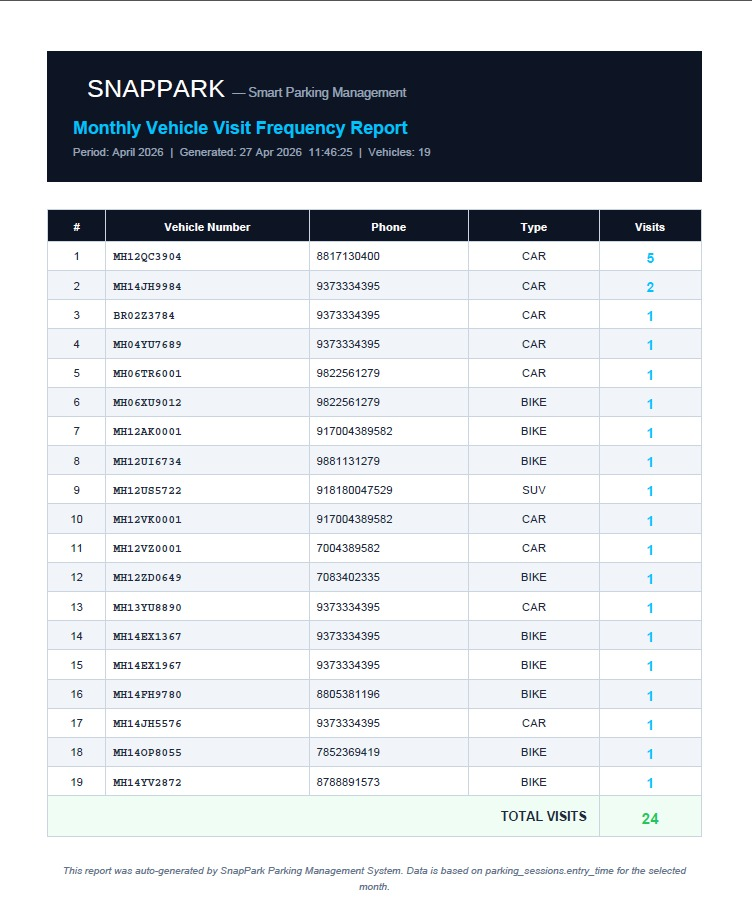
\includegraphics[width=0.85\textwidth]{../images/pdfreport.jpeg}
    \caption{Monthly Vehicle Visit Frequency PDF Report — Generated PDF showing branded header, data table with visit counts sorted by frequency, and total visits summary row.}
    \label{fig:pdfreport}
\end{figure}

As shown in Figure~\ref{fig:pdfreport}, the generated PDF includes a professional SnapPark-branded header, a structured data table with vehicle numbers, phone numbers, types, and visit frequencies, and a total visits summary row with green highlighting.

% ══════════════════════════════════════════════════════════
%  SECTION 4: RESULTS
% ══════════════════════════════════════════════════════════
\section{Results and Outcomes}

\subsection{Features Delivered}

\begin{table}[H]
\centering
\caption{Feature Delivery Status}
\begin{tabular}{|l|c|l|}
\hline
\textbf{Feature} & \textbf{Status} & \textbf{Notes} \\
\hline
VehicleFrequencyRow DTO & \checkmark & Immutable, 4 fields \\
\hline
ReportDAO query & \checkmark & JOIN + GROUP BY + COUNT \\
\hline
PdfReportService & \checkmark & Branded PDF with OpenPDF \\
\hline
REST API endpoint & \checkmark & GET with query params \\
\hline
JavaFX download UI & \checkmark & ComboBoxes + FileChooser \\
\hline
Empty data handling & \checkmark & Shows ``No records'' message \\
\hline
Background threading & \checkmark & Non-blocking UI \\
\hline
\end{tabular}
\end{table}

\subsection{Performance Metrics}

\begin{table}[H]
\centering
\caption{Enhancement Metrics}
\begin{tabular}{|l|l|}
\hline
\textbf{Metric} & \textbf{Value} \\
\hline
New files created & 3 (DTO + DAO + Service) \\
\hline
External dependency added & OpenPDF 1.3.30 \\
\hline
SQL operations & JOIN, GROUP BY, COUNT, ORDER BY \\
\hline
PDF generation time & $<$500ms for typical datasets \\
\hline
Build status & BUILD SUCCESS (0 errors) \\
\hline
\end{tabular}
\end{table}

% ══════════════════════════════════════════════════════════
%  SECTION 5: CONCLUSION
% ══════════════════════════════════════════════════════════
\section{Conclusion}

The Monthly Vehicle Visit Frequency PDF Report enhancement transforms SnapPark from a real-time parking manager into a data-driven platform with exportable analytics. The clean separation of concerns---DTO, DAO, Service, Controller, UI---ensures maintainability and testability. The OpenPDF integration demonstrates practical use of third-party Java libraries in a production system, while the REST API endpoint enables future integrations with external dashboards or management tools.

% ══════════════════════════════════════════════════════════
%  SECTION 6: LEARNING OUTCOMES
% ══════════════════════════════════════════════════════════
\section{Learning Outcomes}

\begin{itemize}
    \item \textbf{DTO Pattern:} Created immutable data transfer objects for clean inter-layer communication.
    \item \textbf{SQL Aggregation:} Implemented complex JOIN + GROUP BY + COUNT queries with PreparedStatements.
    \item \textbf{PDF Generation:} Learned OpenPDF library for programmatic document creation with custom fonts, colors, and table layouts.
    \item \textbf{REST API Design:} Built a binary-response endpoint with proper Content-Type and Content-Disposition headers.
    \item \textbf{JavaFX Threading:} Used background threads with \texttt{Platform.runLater()} for non-blocking UI operations.
    \item \textbf{Dependency Management:} Added and configured external Maven dependencies in \texttt{pom.xml}.
\end{itemize}

\end{document}
